% LaTeX Template for Project Report, Version 2.0
% (Abstracted from a Major Project Report at CSED, NIT Calicut but can be
% modified easily to use for other reports also.)
%
% Released under Creative Commons Attribution license (CC-BY)
% Info: http://creativecommons.org/licenses/by/3.0/
%
% Created by: Kartik Singhal
% BTech CSE Batch of 2009-13
% NIT Calicut
% Contact Info: kartiksinghal@gmail.com
%
% It is advisable to learn the basics of LaTeX before using this template.
% A good resource to start with is http://en.wikibooks.org/wiki/LaTeX/
%
% All template fields are marked with a pair of angular brackets e.g. <title here>
% except for the ones defining citation names in ref.tex.
%
% Empty space after chapter/section/subsection titles can be used to insert text.
%
% Just compile this file using pdflatex after making all required changes.
\documentclass[12pt,a4paper]{report}

% For algorithm
\usepackage{algorithm}
\usepackage[noend]{algpseudocode}

\usepackage[utf8]{inputenc}
\usepackage[french,british]{babel}
\usepackage{amsthm}
\usepackage{amsmath}
\usepackage{amssymb}
\usepackage{verbatim}
\usepackage{caption}
\usepackage{subcaption}
\usepackage{afterpage}
\usepackage{indentfirst}
\let\oldlistofalgorithms\listofalgorithms
\renewcommand{\listofalgorithms}{%
  \begingroup%
  \let\oldnumberline\numberline%
  \renewcommand{\numberline}{Algorithm~\oldnumberline}%
  \oldlistofalgorithms%
  \endgroup}

\usepackage[pdftex]{graphicx} %for embedding images
\usepackage{url} %for proper url entries
\usepackage[bookmarks, colorlinks=false, pdfborder={0 0 0}, pdftitle={Sgd pour la classification d'image}, pdfauthor={Quoc-Khai NGUYEN}, pdfsubject={Sgd pour la classification d'image}, pdfkeywords={sgd}]{hyperref} %for creating links in the pdf version and other additional pdf attributes, no effect on the printed document
%\usepackage[final]{pdfpages} %for embedding another pdf, remove if not required
\usepackage{fancyhdr}
\pagestyle{fancy}

\fancyhead[L]{}



\newlength\mylen
\newcommand\myinput[1]{%
  \settowidth\mylen{\KwIn{}}%
  \setlength\hangindent{\mylen}%
  \hspace*{\mylen}#1\\}


\begin{document}

\begin{otherlanguage}{french}

%\renewcommand\bibname{References}

%include other pages
\begin{titlepage}

\begin{flushright}
ANNÉE 2014\\[1.0cm]
\end{flushright}
\begin{center}
\begin{figure}[!htb]
\minipage{0.18\textwidth}
  
\includegraphics[width=\linewidth]{images/ifi-logo}
\endminipage\hfill
\minipage{0.18\textwidth}
  
\includegraphics[width=\linewidth]{images/auf-logo}
\endminipage\hfill
\minipage{0.18\textwidth}
  
\includegraphics[width=\linewidth]{images/unh-logo}
\endminipage\hfill
\minipage{0.18\textwidth}
  
\includegraphics[width=\linewidth]{images/ctu-logo}
\endminipage\hfill
\end{figure}

Université de Nationale de Hanoi - Agence universitaire de la Francophonie\\
\normalsize
\textsc{Institut de la Francophonie pour l'Informatique}\\[1.0in]
\end{center}

% Title

\begin{flushright}
\Large {\textbf{Algorithme parallèle de \\
Descente de gradient stochastique multi-classes pour la classification d'images}}\\[0.5in]

\line(1,0){250} \\

\normalsize Réalisé par \\
\textbf{Quoc-Khai NGUYEN}\\
Promotion 17 de l'IFI\\[0.5cm]

Sous la direction de \\
{\textbf{Thanh-Nghi DO}}\\
{\textbf{Nguyen-Khang PHAM}}\\
Professeurs de l'Université de Cantho \\[0.5cm]


\vfill

\vspace{0.2cm}

\line(1,0){250} \\
Stage en Master 2 réalisé à la laboratoire de traitement intelligent des informations de la faculté des technologies de l'information et de la communication, Université de Cantho

\end{flushright}
\end{titlepage}

\clearpage
\thispagestyle{empty}

\begin{center}
\huge{Université de Nationale de Hanoi - Agence universitaire de la Francophonie}\\[0.5cm]
\normalsize
\textsc{Institut de la Francophonie pour l'Informatique}\\[2.0cm]
\end{center}

\normalsize Stage en Master 2 réalisé à la laboratoire de traitement intelligent des informations de la faculté des technologies de l'information et de la communication, Université de Cantho.\\[1.0cm]


\begin{flushright}
\line(1,0){250} \\
Réalisé par \\
\textbf{Quoc-Khai NGUYEN}\\
Promotion 17 de l'IFI\\[1.5cm]

Sous la direction de \\
{\textbf{Thanh-Nghi DO}}\\
{\textbf{Nguyen-Khang PHAM}}\\
Professeurs de l'Université de Cantho \\[0.5cm]

\end{flushright}


\clearpage
\thispagestyle{empty}
\begin{large}
Try not to become a man of success, but rather to become a man of value ....
\end{large}

\clearpage
\thispagestyle{plain}
\chapter*{Remerciement}
A lot of people helped me.
\pagenumbering{arabic} %reset numbering to normal for the main content

\cleardoublepage  % \clearpage (if using single side)
\phantomsection
\addcontentsline{toc}{chapter}{Table des matières} \raggedbottom \pagebreak \thispagestyle{empty}
\tableofcontents


\cleardoublepage  % \clearpage (if using single side)
\phantomsection
\addcontentsline{toc}{chapter}{Résumé}
\chapter*{Résumé}
La classification d'images consiste à étiqueter automatiquement des images en catégories prédéfinies. Son application se compose plusieurs domaines importants.\\

Ce projet consiste à étudier les problèmes concernant la classification d'images et à développer un algorithme parallèle multi-classes basé sur la descente de gradient stochastique. Dans un premier temps,  on extrait des données visuelles dans des images. Nous avons d'abord étudié la représentation des images par des vecteurs caractéristiques (SIFT)\cite{low99}. L'étape suivante consiste à construire un vocabulaire visuel en appliquant l'algorithme de clustering, k-moyenne sur un ensemble de vecteurs caractéristiques. Un cluster correspond à un mot visuel. Enfin, une image s'est représentée par un histogramme des mots visuels. Cette approche s'inspire au modèle sac-de-mots largement utilisé dans l'analyse des données textuelles. Dans un second temps, nous nous concentrons sur le problème d'apprentissage automatique basé sur la descente de gradient stochastique. Se basant sur l'implémentation SGD binaire Pegasos dans \cite{sss07}, nous avons développé l'algorithme MC-SGD pour la classification multi-classes. Afin d'améliorer la vitesse de l'algorithme sur des machines multi-cœurs, nous avons aussi parallélisé cet algorithme en utilisant l'OpenMP.\\

Nous constatons que les résultats de notre algorithme sont similaires à ceux de la LibSVM. De plus, notre algorithme est beaucoup plus rapide que la LibSVM, surtout pour les données complexes. Donc, notre méthode s'adapte bien pour la classification d'images où les données sont grandes.

\end{otherlanguage}

\cleardoublepage  % \clearpage (if using single side)
\phantomsection
\addcontentsline{toc}{chapter}{Abstract} \raggedbottom \pagebreak \thispagestyle{empty}
\chapter*{Abstract}
Image classification is to automatically tag images in predefined categories. Its application is made several important domains.\\

This project is to study the problems that concerns the image classification and to develop a parallel multi-class algorithm based on the stochastic gradient descent. Initially, visual data is extracted from images. We first studied the representation of images by feature vectors (SIFT) \cite{low99}. The next step is to construct a visual vocabulary by applying of the clustering algorithm, k-mean on the set of feature vectors. A cluster corresponds to a visual word. Finally, an image is represented by a histogram of visual words. This approach is based on model bag of visual words widely used in the analysis of textual data. In a second step, we focus on the machine learning problem based on the stochastic gradient descent. Based on the implementation binary SGD in Pegasos \cite{sss07}, we have developed the MC-SGD algorithm for multi-class classification. To improve the speed of the algorithm on multi-core machine, we also parallelize the algorithm using OpenMP.\\

We note the results of our algorithm are similar to those of LibSVM. In addition, our algorithm is much faster than LibSVM, especially for complex data. So our method is well suited for image classification where the data are large.

\begin{otherlanguage}{french}
%\afterpage{\null}

\cleardoublepage
\phantomsection
\chapter{Introduction générale}

\section{Introduction}

La classification ou la catégorie des images sont importantes pour accéder à l'information visuelle au niveau d'objets, qui consiste à étiqueter automatiquement des images en catégories prédéfinies. Ces méthodes sont largement utilisées tels que : la reconnaissance des scènes naturelles, la reconnaissance des chiffres sur des chèques, la reconnaissance des codes postaux pour la classification automatique des courriers, la reconnaissance des visages pour l'authentification, etc.\\

Dans ce domaine, le résultat de classification n'est pas très exact. La vitesse d'apprendre des méthode actuelle est base. Fait face de ce problème, on a besoin d'améliorer la vitesse des méthodes ou développer une autre méthode qui est moins compliqué et qui donne le résultat de classification acceptable. La méthode Descente de Gradient Stochastique (SGD) est un bon choix pour ce problème. Donc, ce stage fait le point sur la méthode SGD, MC-SGD et sa version parallèle.

\section{Description par chapitre}

Avant de parler de notre travail, dans premier temps, nous allons présenter la théorie de base des méthodes utilisées. Tout d'abord, nous allons présenter la méthode SIFT et la méthode Sac de Mots dans le chapitre \ref{chap:sift}. Ensuite, nous allons présenter l'étape d'apprentissage automatique qui se compose la méthode SVM standard et une version de SVM avec SGD dans le chapitre \ref{chap:sgd}. Dans ce chapitre, nous parlerons aussi des façons pour résoudre le problème de multi-classes avec un classificateur de 2 classes. Dans le second temps, nous présenterons notre implémentation dans le chapitre \ref{chap:impl}. Pour le chapitre \ref{chap:res}, nous présenterons le résultat obtenue et l'analyserons en détaillé. A la fin de ce rapport, nous terminerons avec la conclusion et perspective dans le chapitre \ref{chap:con}. %literature survey included in this
\chapter[Extraction des caractéristiques]{Extraction des caractéristiques visuelles}
\label{chap:sift}

\section{Introduction}
\newtheorem{mydef}{Définition}
\begin{mydef}
\textbf{Caractéristique visuelle} \\
Une caractéristique d'une image est définie comme une abstraction des informations visuelles de l'image qui sont sélectionnée pour des tâches de calcul reliées à une certaine application (par ex : classification d'images, recherche d'images).
\end{mydef}

Les caractéristiques sont extraites soit globalement sur une image entière, soit sur une petite groupe de pixel (une région) d'une image. Le résultat d'une étape d'extraction de caractéristiques (globales ou locales) est appelé \textit{descripteur de caractéristiques.}

\begin{mydef}
\textbf{Descripteur de caractéristiques} \\
Nous appelons la description mathématique d'une image ou une région locale de l'image après une étape d'extraction de caractéristiques sont \textbf{descripteur de caractéristiques}
\end{mydef}

Les descripteurs se présentent normalement sous forme d'une vecteur dans un espace vectoriel, $\mathbb{R}^D$, appelé \textit{l'espace de caractéristiques}. \\

Dans le cas d'une extraction globale, on récupère une seule descripteur par image tandis qu'une description locale permet d'obtenir d'un ensemble de descripteur locaux pour une image. \\

Jusqu'à maintenant, les cherches se basent plusieurs types de caractéristiques pour la classification ou la reconnaissance d'images. Nous pouvons lister quelques types de caractéristiques les plus couramment utilisées pour calculer des descripteur : \textit{la couleur, la texture, la forme, les points d'intérêt et les relations spatiales} qui sont décrit dans \cite{khang09}.\\

\section{Description locale des images}
Afin d'obtenir des descripteur locaux à partir une image, on commence par extraire des régions. La façon la plus simple est d'utiliser une \textit{partition} qui découpe l'image en rectangles ou en cercles de même taille. Une telle partition simple ne génère pas de région perceptuelle-ment significatives mais c'est une manière simple d'obtenir des caractéristiques globales de l'image avec une résolution plus fine. Dans la lecture, nous trouvons que les deux approches les plus utilisées pour localiser les région d'intérêt dans l'image : l'une fournit des régions qui se chevauchent (détection des points d'intérêt) et l'autre segmente l'image en région sans intersection (segmentation d'image)\cite{khang09}. La première approche est efficace pour la classification d'images, donc, dans cette section nous décrivons la première approche.\\[0.5cm]
\textbf{Détection des points d'intérêt}\\
Les points d'intérêt sont traditionnellement utilisés pour la \textit{stéréo vision} mais sont utilisés aussi dans la classification d'images. Ils sont déterminés de manière telle qu'un point trouvé dans une image sera aussi trouvé dans une autre image qui diffère légèrement de la première. La signification de tels points spéciaux est due à leur représentation compacte des régions importantes de l'image qui conduit à une indexation efficace, et à leur pouvoir discriminant surtout dans la recherche d'objets.\\

Un des premiers travaux sur ce sujet \cite{sm97} utilise un détecteur de Harris \cite{hs88} pour localiser des points d'intérêt invariants à la rotation. Dans \cite{dsh00}, les auteurs montrent que les descripteurs ne peuvent pas être invariants au changement d'échelle si les points d'intérêt extraits ne sont pas invariants eux même au changement d'échelle. Par conséquent, plusieurs détecteurs ont été proposé pour obtenir l'invariance au changement d'échelle des points d'intérêt \cite{lin98, low99, ms01, low04}. La sélection automatique de l'échelle est effectuer en choisissant les \textit{extrema} d'une fonction de l'échelle (par ex. laplacien normalisé, différence de gaussiennes).\\[0.5cm]
\textbf{Caractérisation des points d'intérêt}\\
Après avoir détecté des points d'intérêt, pour les utiliser, il faut caractériser la région autour de ces points. La caractérisation d'un point d'intérêt est calculée, à une échelle choisie, sur la région autour de ce point. Différents descripteurs ont été proposés dans la littérature : \textit{Shape context} \cite{bmp02}, \textit{Scale Invariant Feature Transform (SIFT)} \cite{low04}, \textit{PCA-SIFT} \cite{ks04}, \textit{Gradient Location and Orientation Histogram (GLOH)} \cite{ms05}. Parmi des descripteurs listés, le descripteur SIFT est le plus utilisé \cite{khang09}. Dans ce travail, nous concentrerons au descripteur SIFT, donc, nous décrivons ce descripteur et cette méthode dans la partie ci-dessous.

\section{Méthode SIFT (Scale-invariant feature transform)}
\subsection{Introduction}
Dans la lecture, nous trouvons qu'on traduit en français "transformation de caractéristiques visuelles invariante à l'échelle". SIFT est une méthode utilisé dans le domaine de la vision par ordinateur pour détecter et identifier les éléments similaires entre différentes images numériques (éléments de paysages, objets, personnes, etc.). Cette méthode a été développé en 1999 par le chercheur David Lowe \cite{low99}.\\

L'étape fondamentale de la méthode SIFT consiste à calculer les \textit{descripteurs SIFT} des images à étudier. Il s'agit d'informations numériques dérivées de l'analyse locale d'une image et qui caractérisent le contenu visuel de cette image de la façon la plus indépendante possible de l'échelle, du cadrage, de l'angle d'observation et de l'exposition (luminosité) \cite{low99}.\\

La méthode proposée par Lowe comprend deux parties \cite{low04}~:
\begin{enumerate}
\item un algorithme de détection de caractéristiques et de calcul de descripteurs
\item un algorithme de mise en correspondance proprement dit
\end{enumerate}
De ces deux aspects, le premier est celui qui a le plus assuré la popularité de la méthode \cite{mt10}. La deuxième permet d'utiliser le résultat de la première partie pour l'usage de la méthode. Dans notre travail, nous utilisons la méthode SIFT comme un résultat de base. C'est à dire, nous n'utilisons que la première partie de la méthode.\\

La première partie, partie de détection de caractéristiques et de calculer des descripteurs comprend 4 étapes principales \cite{low99, low04}~:
\begin{enumerate}
\item Détection d'extrema dans l'espace des échelles.
\item Localisation précise de points d'intérêt
\item Assignation d'orientation
\item Descripteur de point d'intérêt
\end{enumerate}
Nous décrivons tout de suite pas à pas ces étapes.

\subsection{Détection d'extrema dans l'espace des échelles}
La détection s'effectue dans un espace discret (espace des échelles ou \textit{scale space} en anglais) qui comporte trois dimensions : les coordonnées cartésiennes $x$ et $y$ et le facteur d'échelle $\sigma$. Le gradient de facteur d'échelle $\sigma$ (noté $L$) est le résultat de la convolution d'une image $I$ par un filtre gaussien $G$ de paramètre d'échelle $\sigma$, soit \cite{low04} :

\begin{equation}
L \left( x, y, \sigma \right) = G \left( x, y, \sigma \right) * I \left( x, y \right)
\end{equation}
Et
\[
G \left( x, y, \sigma \right) = \frac{1}{2\pi\sigma^2}
\]

Cette convolution a pour effet de lisser l'image originale $I$ de telle sorte que les détails trop petits, c'est-à-dire de rayon inférieur à \footnote{ Ici comme dans la littérature scientifique en général, le facteur d'échelle – paramètre du filtre gaussien $\sigma$ – est assimilé à une distance en pixels sur l'image, que l'on pourrait appeler rayon associé $r$. En fait, ils sont proportionnels ($r = \alpha \sigma$), avec un facteur $\alpha$ qui varie généralement entre 3 et 4 selon les auteurs. Il est tout simplement lié au nombre de coefficients au-delà duquel les valeurs de la gaussienne deviennent négligeables.}, sont estompés. Par conséquent, la détection des objets de dimension approximativement égale à $\sigma$ se fait en étudiant l'image appelée différences de gaussiennes (en anglais difference of gaussians, DoG) définie comme suit :
\begin{equation}
D \left( x, y, \sigma \right) = L \left( x, y, k\sigma \right) - L \left( x, y, \sigma \right)
\end{equation}
Ou
\[
D \left( x, y, \sigma \right) = (G \left( x, y, k\sigma \right) - G \left( x, y, \sigma \right)) * I \left( x, y \right)
\]

où $k$ est un paramètre fixe de l'algorithme qui dépend de la finesse de la discrétisation de l'espace des échelles voulue \cite{low04}.\\

Pour chaque octave de l'espace des échelle, l'image initiale répétée est fait la convolution avec gaussiennes pour produire l'ensemble des images de l'espace des échelle (image ci-dessous, à gauche). Images gaussiennes adjacentes sont soustraites
pour produire les images de différence de gaussienne sur la droite. Après chaque octave, l'image Gaussian est sous-échantillonnée par un facteur de 2, et le processus est répété pour toutes les échelle.

\begin{figure}[ht!]
\centering
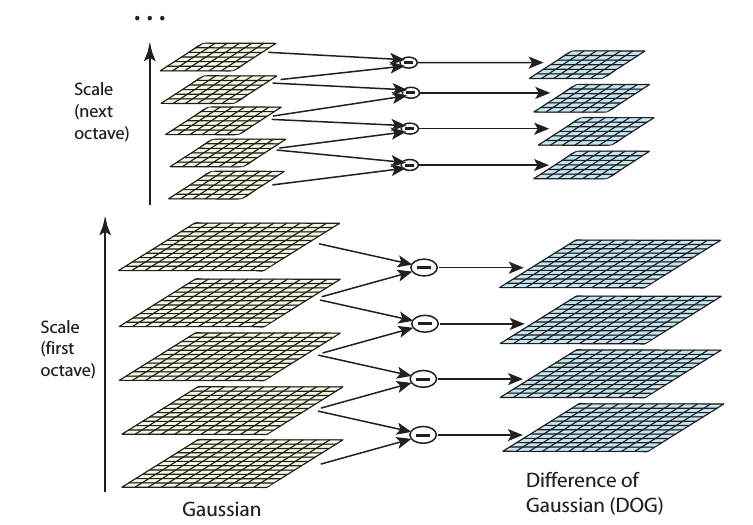
\includegraphics[width=150mm]{images/dog}
\caption{Différence de Gausienne \cite{low04}}
\label{overflow}
\end{figure}

Un point d'intérêt candidat ($x,y,\sigma$) est défini comme un point où un extremum du DoG est atteint par rapport à ses voisins immédiats, c'est-à-dire sur l'ensemble contenant 26 autres points défini par~:
\[
\{ D \left( x + \delta_x, y + \delta_y, s \sigma \right), \delta_x \in \{-1, 0, 1\}, \delta_y \in \{-1,0, 1\}, s \in \{k^{-1}, 1, k\} \} 
\]
On peut voir l'image ci-dessous pour être facile à comprendre
\begin{figure}[ht!]
\centering
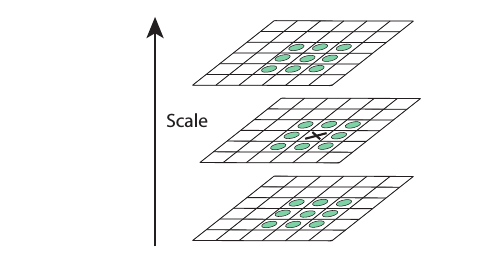
\includegraphics[width=100mm]{images/select_point}
\caption{\cite{low04} Le maxima et le minima des images de différence de gaussienne sont détectés en comparant une
pixel (marqué X) à ses 26 voisins dans les régions de 3x3 aux échelles actuels et adjacents (marqué avec des cercles).}
\label{overflow}
\end{figure}

\pagebreak
\subsection{Localisation précise de points d'intérêt}
L'étape de détection d'extremums produit en général un grand nombre de points-clés candidats, dont certains sont instables. De plus, leur localisation, en particulier aux échelles les plus grandes (autrement dit dans les octaves supérieures de la pyramide où la résolution est plus faible) reste approximative. De ce fait, des traitements supplémentaires sont appliqués, pour un objectif double : d'une part, reconverger la position des points pour améliorer la précision sur $x$, $y$ et $\sigma$, d'autre part, éliminer les points de faible contraste ou situés sur des arêtes de contour à faible courbure et donc susceptibles de "glisser" facilement.

\subsection{Assignation d'orientation}
L'étape d'assignation d'orientation consiste à attribuer à chaque point-clé une ou plusieurs orientations déterminées localement sur l'image à partir de la direction des gradients dans un voisinage autour du point. Dans la mesure où les descripteurs sont calculés relativement à ces orientations, cette étape est essentielle pour garantir l'invariance de ceux-ci à la rotation : les mêmes descripteurs doivent pouvoir être obtenus à partir d'une même image, quelle qu'en soit l'orientation\cite{low04}.

Pour un point-clé donné ( $x_0$, $y_0$, $\sigma_0$ ), le calcul s'effectue sur $L ( x, y, \sigma_0 )$, à savoir le gradient de la pyramide dont le paramètre est le plus proche du facteur d'échelle du point. De cette façon, le calcul est également invariant à l'échelle. À chaque position dans un voisinage du point-clé, on estime le gradient par différences finies symétriques, puis son amplitude (c.-à-d. sa norme) $m ( x, y )$, et son orientation $\theta ( x, y )$ \cite{low04}~:

\begin{equation}
m \left( x, y \right) = \sqrt{\bigl( L \left( x+1, y \right) - L \left( x-1, y \right) \bigr)^2 + \bigl( L \left( x, y+1 \right) - L \left( x, y-1 \right) \bigr)^2}
\end{equation}

\begin{equation}
\theta \left( x, y \right) = \tan^{-1}\left(\frac{L \left( x, y+1 \right) - L \left( x, y-1 \right)}{L \left( x+1, y \right) - L \left( x-1, y \right)} \right)
\forall\left(x, y\right) \hbox{ dans un voisinage de } \left(x_0, y_0\right)
\end{equation}

Un histogramme des orientations sur le voisinage est réalisé avec 36 intervalles, couvrant chacun 10 degrés d'angle. L'histogramme est doublement pondéré : d'une part, par une fenêtre circulaire gaussienne de paramètre égal à 1,5 fois le facteur d'échelle du point-clé $\sigma_0$, d'autre part, par l'amplitude de chaque point. Les pics dans cet histogramme correspondent aux orientations dominantes. Toutes les orientations dominantes permettant d'atteindre au moins 80\% de la valeur maximale sont prises en considération, ce qui provoque si nécessaire la création de points-clés supplémentaires ne différant que par leur orientation principale\cite{low04}.

\begin{figure}[ht!]
\centering
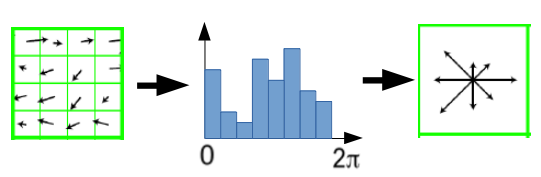
\includegraphics[width=100mm]{images/sift_hist}
\caption{Illustration de la construction de l'histogramme des orientations}
\label{overflow}
\end{figure}

À l'issue de cette étape, un point-clé est donc défini par quatre paramètres $( x, y, \sigma, \theta )$. Il est à noter qu'il est parfaitement possible qu'il y ait sur une même image plusieurs points-clés qui ne différent que par un seul de ces quatre paramètres (le facteur d'échelle ou l'orientation, par exemple).


\subsection{Descripteur de point d'intérêt}
Une fois les points-clés, associés à des facteurs d'échelles et à des orientations, détectés et leur invariance aux changements d'échelles et aux rotations assurée, arrive l'étape de calcul des vecteurs descripteurs, traduisant numériquement chacun de ces points-clés. À cette occasion, des traitements supplémentaires vont permettre d'assurer un surcroît de pouvoir discriminant en rendant les descripteurs invariants à d'autres transformations telles que la luminosité, le changement de point de vue 3D, etc. Cette étape est réalisée sur l'image lissée avec le paramètre de facteur d'échelle le plus proche de celui du point-clé considéré\cite{low04}.
\begin{figure}[ht!]
\centering
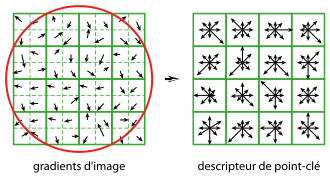
\includegraphics[width=100mm]{images/siftdescriptor}
\caption{Construction d'un descripteur SIFT}
\label{overflow}
\end{figure}

Autour de ce point, on commence par modifier le système de coordonnées local pour garantir l'invariance à la rotation, en utilisant une rotation d'angle égal à l'orientation du point-clé, mais de sens opposé. On considère ensuite, toujours autour du point-clé, une région de $16x16$ pixels, subdivisée en $4x4$ zones de $4x4$ pixels chacune. Sur chaque zone est calculé un histogramme des orientations comportant 8 intervalles. En chaque point de la zone, l'orientation et l'amplitude du gradient sont calculés comme précédemment. L'orientation détermine l'intervalle à incrémenter dans l'histogramme, ce qui se fait avec une double pondération par l'amplitude et par une fenêtre gaussienne centrée sur le point clé, de paramètre égal à 1,5 fois le facteur d'échelle du point-clé\cite{low04}.\\

Ensuite, les 16 histogrammes à 8 intervalles chacun sont concaténés et normalisés. Dans le but de diminuer la sensibilité du descripteur aux changements de luminosité, les valeurs sont plafonnées à 0,2 et l'histogramme est de nouveau normalisé, pour finalement fournir le descripteur SIFT du point-clé, de dimension 128.

\section{Méthode BoW (Bag of word)}
La représentation par sac de mots \textit{(ou bag of words en anglais)} est une description de document (texte, image, ...) très utilisée en recherche d'information. Spécialement, dans la classification d'images, cette méthode est largement utilisée après l'étape d'extraction des descripteurs. Dans DoW, les méthodes de cluster sont utilisées pour grouper des  descripteurs. Actuellement, la méthode K-moyenne (Kmeans)\cite{jm67} est beaucoup utilisée pour grouper des des descripteurs SIFT aux clusters, chaque cluster est considère comme un mot visuel, l'ensemble de mots visuels jouent le rôle d'un dictionnaire de mots visuels. Ensuite, BoW met chaque descripteur de chaque image au cluster qui est le plus proche( se base sur la distance entre chaque descripteur et sa future cluster ). Suite, chaque image est décrite comme un histogramme des mots. Cette méthode est décrite comme l'image ci-dessous.

\begin{figure}[ht!]
\centering
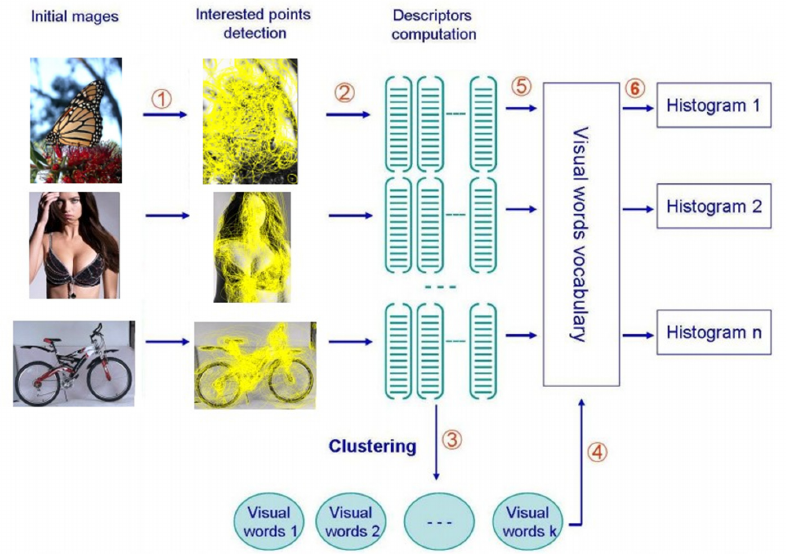
\includegraphics[width=160mm]{images/bow}
\caption{Model de BOW}
\label{overflow}
\end{figure}

\chapter{Apprentissage automatique}
\label{chap:sgd}

\section{Introduction}
L'apprentissage automatique (machine learning) est un domaine de l'intelligence artificielle, qui permet aux machines d'apprendre à partir des données. L'apprentissage automatique est la discipline scientifique concernée par le développement, l'analyse et l'implémentation de méthodes automatisables qui permettent à une machine d'évoluer autonome-ment grâce à un processus d'apprentissage, et ainsi de remplir des tâches qu'il est difficile ou impossible de remplir par des moyens algorithmiques plus classiques. Le problème ici est que la donnée d'observation est petite, elle ne peut pas comprendre tout l'ensemble de données d'entrées (tous les cas) qui est trop grande. Un programme d'apprentissage automatique doit généraliser des données limite afin de données des réactions intelligentes sur des nouveaux exemples.\\

\section{Méthode SVM (Support Vector Machine)}
Les machines à vecteurs de support (Support Vector Machine, SVM) sont un ensemble de techniques d'apprentissage supervisé destinées à résoudre des problèmes de classification et de régression. Dans cette section, nous ne parlons que SVM pour la classification concernant notre projet dans la pratique.\\

La méthode SVM cherche l'hyperplan optimal qui permet de séparer les points (les données) en deux parties en respectant le principe où les points d'une même classe doit être dans la même partie (classification de 2 classes). Pour les problème de classification multi-classes, on a des méthodes pour qu'il devient la problème de 2 classes que nous parlerons dans la partie MC-SGD.
\begin{figure}[ht!]
\centering
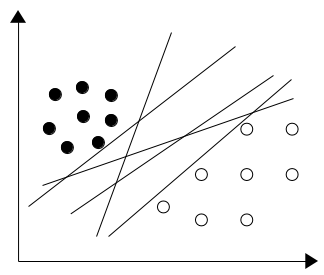
\includegraphics[width=55mm]{images/separating_lines}
\caption{Classification linéaire}
\label{slines}
\end{figure}

Le cas simple est le cas d'une fonction de classification linéaire comme dans l'image \ref{slines}. On a $m$ exemples d'entrées $x_1, x_2, ..., x_m$ dans l'espace de $N$ dimensions. Chaque exemple $x_i$ a un label $y_i$ : $y_1, y_2, ..., y_m$ $(y_i \in \{-1,1\})$. Plusieurs hyperplans peuvent séparer ces 2 classes, mais SVM cherche l'hyperplan optimal qui est défini comme l'hyperplan qui maximise la marge entre les échantillons et l'hyperplan séparateur. La marge est la distance entre l'hyperplan et les échantillons les plus proches. Ces derniers sont appelés \textit{vecteurs supports}. Dans l'espace de \textit{N} dimensions, l'hyperplan est défini par le vecteur $w=[w_1,w_2,...,w_n]$ et $b$. SVM cherche l'hyperplan $(w, b)$ pour classifier les données comme l'image \ref{max_margin} :

\begin{figure}[ht!]
\centering
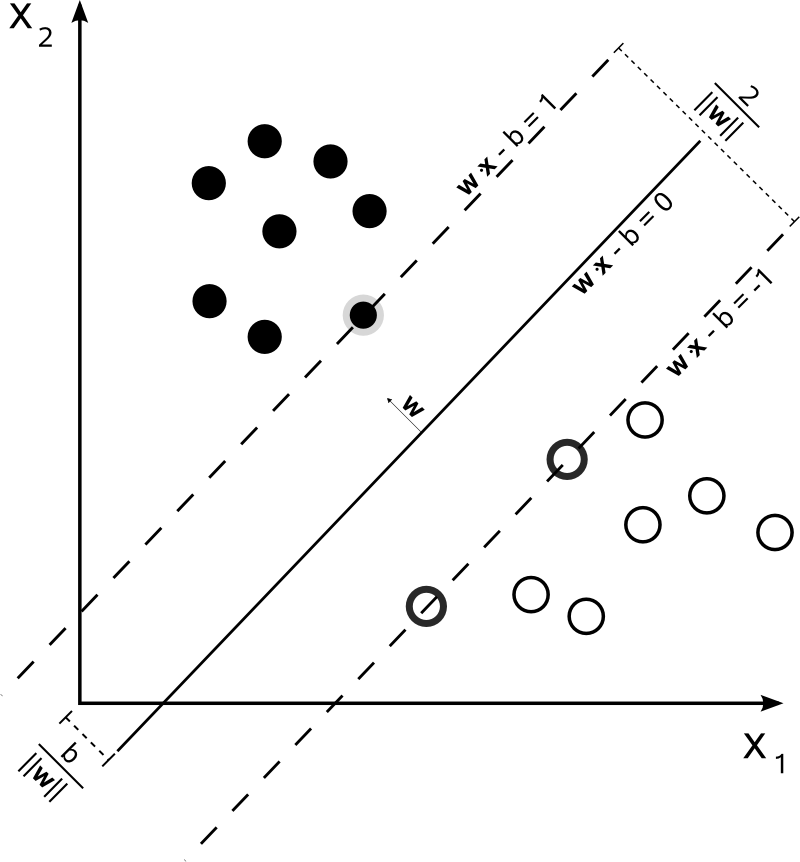
\includegraphics[width=55mm]{images/margin}
\caption{L'hyperplan optimal}
\label{max_margin}
\end{figure}

Après avoir trouvé $w$ et $b$, l'hyperplan optimal est défini : $x^T.w - b = 0$ et 2 supports hyperplans $x^T.w - b = 1$ et $x^T.w - b = -1$. Par rapport à 2 supports hyperplans parallèles (voir l'image \ref{max_margin}), la classification est réalisée grâce aux \ref{f1} et \ref{f2}.
\begin{equation}
x_i.w - b \geq +1, \Rightarrow y_i = 1
\label{f1}
\end{equation}

\begin{equation}
x_i.w - b \leq -1, \Rightarrow y_i = -1
\label{f2}
\end{equation}

La classification peut être expliqué : l'hyperplan supporte la classe \textit{\textbf{(+1)}} est l'hyperplan que les points qui a le label \textit{\textbf{(+1)}} au dessus de l'hyperplan. Comme ça, l'hyperplan supporte la classe \textit{\textbf{(-1)}} est l'hyperplan que les points qui a le label \textit{\textbf{(-1)}} au dessous de l'hyperplan. Par rapport aux \ref{f1} et \ref{f2}, on a le formule \ref{f3}

\begin{equation}
y_i.(x_i.w - b) \geq 1
\label{f3}
\end{equation}

Dans le cas où l'algorithme ne peut pas trouver $(w, b)$ satisfait le problème (les données sont inséparable), nous devons accepter des erreurs $z_i$. Chaque exemple $i$ est dans son vrais hyperplan, son erreur $z_i = 0$, sinon, son erreur $z_i$ est défini par la distance entre cet exemple et son hyperplan. Le formule \ref{f3} devient \ref{f4} :

\begin{equation}
y_i.(x_i.w - b) + z_i \geq 1
\label{f4}
\end{equation}

Nous trouvons que la classification est facile si l'on a trouvé $w$ et $b$. La difficulté de la méthode SVM est que comment trouver $w$ et $b$. Ce tache est réalisé après avoir trouvé la solution du programme de quadratique \ref{f5}.

\begin{equation}
\begin{split}
\mbox{min}\quad \Psi(w, b, z) = \frac{1}{2} ||w||^2 + c.\sum\limits_{i=1}^m z_i\quad \\ \mbox{s.t} \quad y_i.(x_i.w - b) + z_i \geq 1 \\ \mbox{and} \quad z_i \geq 0
\end{split}
\label{f5}
\end{equation}

Le problème d'optimisation quadratique \ref{f5} est un des problèmes d'optimisation qui est normalement recherché dans le domaine de mathématique d'optimisation. Pour l'implémentation ce problème, \cite{jp98} et \cite{cl01} ont la complexité de $O(N^2)$ (N est le nombre d'exemples). Ce sont des programmes les plus utilisés actuel.

\section{Méthode SVM avec SGD (Stochastic gradient descent)}
SVM standard est efficace mais la complicité est grande $(O(N^2))$, donc, c'est intraitable pour les larges données. La méthode SVM avec SGD (Stochastic Gradient Descent), ou pour plus sample, on appelle la méthode SGD est créées pour résoudre ce problème. SGD ne cherche pas la solution pour résoudre le problème du programme de quadratique. Cette méthode ignore $b$  dans le formule \ref{f5}. Le contraint $y_i.(x_i.w - b) + z_i \geq 1$ peut être remplacé par : 

\begin{equation}
z_i \geq 1 - y_i.(x_i.w)
\label{f6}
\end{equation}

A partir du contraint \ref{f6} et $z_i \geq 0$, on peut écrire la function de perte :

\begin{equation}
z_i = max\lbrace0, 1 - y_i.(x_i.w)\rbrace
\label{f7}
\end{equation}

Donc, le programme de quadratique \ref{f5} peut remplacer par le formule \ref{f8} :

\begin{equation}
\mbox{min}\quad \Psi(w, x, y) = \frac{1}{2} ||w||^2 + \frac{1}{m}\sum\limits_{i=1}^m max\lbrace0, 1 - y_i.(x_i.w)\rbrace\quad
\label{f7}
\end{equation}

Cette méthode est proposée dans \cite{sss07}. Dans cette méthode, $w$ est mise à jour en T étapes avec une vitesse d'apprentissage $\eta$. A chaque étape $t$, SGD utilise un exemple $(x_i, y_i)$ aléatoire pour calculer le sous-gradient et met à jour $w_{t+1}$. 

\begin{equation}
w_{t+1} = w_t - \nabla_w{\Psi(w_t, x_i, y_i)}
\label{f8}
\end{equation}
\\

Cette algorithme est linéaire avec le nombre d'exemple. C'est la raison pour laquelle il est beaucoup plus vite que SVM standard. 

%Nous avons tester avec les données \textit{gisette} \cite{svmdata1} de 10 classes, 60.000 exemples et de 780 caractéristiques par exemple. 


\section{Méthode MC-SGD (Multi Class - Stochastic gradient descent)}
Plupart d'algorithme de SVM ne traite que le problème de 2 classes (binaire). Il existe plusieurs extensions d'une classification binaire afin de traiter le problème de multi-class classification. Actuellement, on a deux façon pour traiter ce problème. L'une considère directement à résoudre le problème de multi-classes \cite{ww99, yg07}. L'autre divise d'abord le problème en plusieurs problèmes de 2 classes et chaque problème de 2 classes est traité par la classification binaire comme one-versus-one \cite{vv95} et one-versus-all \cite{uk99}. \\

En pratique, one-vs-one et one-vs-all sont beaucoup utilisés par leur simple. one-vs-one construit \textit{k(k-1)/2} (k est le nombre de classes) classificateurs, c'est à dire, il utilise tous les paires de classes différents pour l'apprentissage. La prédiction est réalisée par voter et la majorité classificateur va être choisi et la classe correspondant est la classe de prédiction. One-vs-all construit \textit{k} classificateurs, à chaque classificateur \textit{c}, il divise la classes \textit{c} contre tous les restes. La classe de prédiction est la classe ayant la distance la plus courte entre son classificateur et l'exemple d'entrée. \\

Chaque méthode a l'avantage et l'inconvénient. One-vs-one est balancé mais il construit beaucoup de classificateurs. Par contre, one-vs-all construit moins classificateur mais il n'est pas balancé.
\chapter{Implémentation}
\label{chap:impl}

\section{Introduction}
Dans le chapitre précédent, nous avons généralement présenté des méthodes concernant notre travail. Après avoir étudié des différentes méthodes, dans chaque étape, nous avons choisi une méthode qui peut mieux adapter à notre travail. Durant notre recherche, il existe déjà des codages qui a la performance efficace, donc, nous avons réutilisé ces codages. Au contrait, pour les étapes qui n'existent pas encore des codages, nous avons les implémenté nous-même ou nous avons modifié des codages qui n'ont bien adapté pas à notre travail.

\section{Représentation par des descripteurs et méthode sac de mots}
La description des images est très importante dans la classification d'images. Cette étape est beaucoup influencée au résultat final. Dans le domaine de recherche d'images et de classification d'images, le descripteur SIFT \cite{low04} est un caractéristique important pour la représentation des images. Cette méthode est de plus en plus populaire. A partir de l'idée de la classification de textes, dans la recherche en 2007 \cite{bos07}, les auteurs proposent un système de classification d'images utilisant le descripteur SIFT et le modèle sac de mot visuel (Bag of Visual Word). Cette méthode peut diviser en 3 étapes :
\begin{enumerate}
\item Trouver des descripteurs locales des images (des caractères)
\item Construire un dictionnaire a partir des caractères
\item Représenter des images par des histogrammes
\end{enumerate}

Dans ces étapes, nous avons réutilisé des codages existant en modifiant des entrées et des sorties pour adapter aux étapes suivantes. Précisément, dans l'étape \textit{1}, nous avons réutilisé le codage de D.Lowe \cite{low99} pour créer des vecteurs de caractéristiques (descripteurs). Ensuite, l'étape \textit{2} sert à construire un dictionnaire. Dans cette étape, la méthode k-moyenne \cite{mq67} est appliquée afin de créer des clusters a partir des vecteurs SIFT créés dans l'étape \textit{1}. L'ensemble de clusters est considéré comme un dictionnaire. Enfin, dans l'étape \textit{3}, une image est représentée par un histogramme. Dans cette étape, d'abord, on met chaque vecteur SIFT dans chaque image à un cluster le plus proche de ce vecteur (sa base sur la distance entre ce vecteur au centre des clusters). Ensuite, on compte le fréquence des mots d'une image existe dans le dictionnaire créé dans l'étape \textit{2} pour représenter l'image comme un histogramme de fréquence. Pour l'étape \textit{3}, nous avons implémenté en C/C++.

\section{Apprentissage automatique}
Avec notre processus, après la méthode sac de mot visuel, nous appliquons un algorithme d'apprentissage pour classifier des images vers leurs classes. Nous avons développé la méthode MC-SGD et pour vérifier la performance de notre méthode, nous avons fait la comparaison avec l'application LIBSVM \cite{cl01}, l'implémentation de SVM le plus utilisée actuellement.

\subsection{Descente de gradient stochastique (SGD)}
Pour cette méthode, il existe plusieurs d'implémentations différentes. Dans notre travail, nous avons réutilisé l'implémentation \textit{Pegasos} \cite{sss07} ci-dessous :

\begin{algorithm}[H]
\caption{L'algorithm d'apprentissage SGD-SVM binaire}\label{sgdal}
\begin{algorithmic}[1]
\Procedure{trainBinaireSGDSVM}{$D$, $y$, $\lambda$, $T$, $n$}

\State Initialiser $w_1 = 0$

\For{\texttt{t = 0; t < T; t++}}

\State $\eta = \frac{1}{\lambda}$

\Comment{Boucle pour choisir ex exemples chaque cycle}
\For{\texttt{ex = 0; ex < n; ex++}}
\State \texttt{choisir un exemple aléatoire dans D}
\If{\texttt{${y_i}_t.(w_t,{x_i}_t) < 1$}}
\State $w_{t+1} = (1 - \eta_t.\lambda).w_t + \eta_t.{y_i}_t.{x_i}_t$
\Else
\State $w_{t+1} = (1 - \eta_t.\lambda).w_t$
\EndIf
\EndFor

\EndFor

\State Return $w_{t}$

\EndProcedure
\end{algorithmic}
\end{algorithm}



\subsection{Descente de gradient stochastique pour multi-classe (MC-SGD)}
Comme les autres algorithme de SVM, SGD est implémenté pour résoudre le problème de classification de 2 classes. L'implémentation \textit{Pegasos} \cite{sss07} est efficace. A partir de cette implémentation, nous les avons modifié et développé pour résoudre le problème de multi-classes (k classes, $k \geq 3$). \\

Pour le problème de classification de multi-classes, comme nous avons expliqué dans la partie précédente, nous avons utilisé la méthode \textit{one-vs-all}. Cette méthode ne construit que k classificateur (k est le nombre de classes). Par exemple, quand le problème a trois classes comme l'image \ref{mclass}. \textit{One-vs-all} va construire trois classificateurs comme l'image \ref{1vsall}.



\makeatletter
\def\BState{\State\hskip-\ALG@thistlm}
\makeatother


\begin{algorithm}[H]
\caption{L'algorithm d'apprentissage SGD-SVM pour multi-classes}\label{mcsgdal}
\begin{algorithmic}[1]
\Procedure{trainMCSGDSVM}{$D$, $y$, $k$, $\lambda$, $T$, $n$}

\Comment{D est les données d'apprentissage }\\
\Comment{y est les labels des données }\\
\Comment{k est le nombre de classes dans D}\\
\Comment{$\lambda$ est le constant possible }\\
\Comment{T est le nombre de cycles }\\
\Comment{n est le nombre d'exemple par cycle }\\

\State Initialiser k modèles w

\For{\texttt{c = 0; c < k; c++}}\\
\Comment{Préparation des données pour one-vs-all}
\State \texttt{$y_i = +1$ si l'exemple de classe c, $y_i = -1$ sinon}
\State \texttt{$w_c = trainBinaireSGDSVM(D, y, \lambda, T, n)$} $(c-vs-all)$
\EndFor

\State Return $w$

\EndProcedure
\end{algorithmic}
\end{algorithm}


\subsection{Balance de MC-SGD}
Nous trouvons que notre processus est acceptable, one-versus-all s'adapte bien pour la classification multi-classes. Malheureusement, pour les base de données se compose de beaucoup de classes. Par exemple, si le problème de 1000 classes, on a 1 exemple positive et 999 exemple négatives. Chaque fois SGD choisit aléatoire un exemple pour d'apprendre, les exemples positives sont rarement choisi (probabilité de \emph{0.1\%}) mais les exemples négatives sont très souvent choisi (probabilité de \emph{99.9\%}). Donc, le résultat de classification est influencé ! C'est la raison pour laquelle on a besoin d'augmenter la probabilité de sélectionné l'exemple positive. Au lieu de choisir aléatoire un exemple pour d'apprendre, l'algorithme choisit aléatoire entre -1 et +1, si +1 est choisi, SGD choisit aléatoire un exemple pour dans l'ensemble d'exemple positive et inverse.

\begin{algorithm}[H]
\caption{L'algorithm d'apprentissage SGD-SVM binaire balancé}\label{balance-sgdal}
\begin{algorithmic}[1]
\Procedure{trainBinaireSGDSVM}{$D$, $y$, $\lambda$, $T$, $n$}

\State Initialiser $w_1 = 0$

\For{\texttt{t = 0; t < T; t++}}

\State $\eta = \frac{1}{\lambda}$

\Comment{Boucle pour choisir ex exemples chaque cycle}
\For{\texttt{ex = 0; ex < n; ex++}}
\State \texttt{choisir aléatoire entre +1 et -1}
\If{+1 est choisi}
\State \texttt{choisir un exemple positive aléatoire dans D}
\Else
\State \texttt{choisir un exemple négative aléatoire dans D}
\EndIf

\If{\texttt{${y_i}_t.(w_t,{x_i}_t) < 1$}}
\State $w_{t+1} = (1 - \eta_t.\lambda).w_t + \eta_t.{y_i}_t.{x_i}_t$
\Else
\State $w_{t+1} = (1 - \eta_t.\lambda).w_t$
\EndIf
\EndFor

\EndFor

\State Return $w_{t}$

\EndProcedure
\end{algorithmic}
\end{algorithm}




\subsection{Parallélisation de MC-SGD}
Nous trouvons que l'algorithme \ref{mcsgdal} linaire, il apprend les modèles l'un après l'autre sur un seul cœur du processeur d'ordinateur. Donc, les autres cœurs ne font rien et l'algorithme est lent. A notre époque, nous pouvons utiliser tous les cœurs possibles pour améliorer la vitesse de notre algorithme en utilisant la programmation parallèle.\\

Pour le problème de multi-classes (k classes), l'algorithme SGD-SVM apprend indépendant chaque classificateur. Donc, c'est possible d'apprendre chaque classificateur sur chaque cœur différent. Dans notre implémentation, nous avons parallélisé la boucle sur l'apprentissage des classificateur. Supposons que nous avons p processeurs et k classificateurs. Donc, chaque processeur apprend $n = \frac{k}{p}$ ou $n = \frac{k}{p} + 1$ classificateurs.

\begin{algorithm}[H]
\caption{L'algorithm d'apprentissage SGD-SVM parallèle pour multi-classes}\label{pmcsgdal}
\begin{algorithmic}[1]
\Procedure{trainMCSGDSVMParallel}{$D$, $y$, $k$, $\lambda$, $T$, $n$}

\State Initialiser k modèles w
\\
\BState \textbf{Pocesseur 1:}
\State \texttt{$y_i = +1$ si l'exemple de classe c (c = 1, classe 1.p + 1, classe 2.p + 1, ...) et $y_i = -1$ sinon}
\State \texttt{$w_c = trainBinaireSGDSVM(D, y, \lambda, T, n)$} $(c-vs-all)$
\\
\BState \textbf{Pocesseur 2:}
\State \texttt{$y_i = +1$ si l'exemple de classe c (c = 2, classe 1.p + 2, classe 2.p + 2, ...) et $y_i = -1$ sinon}
\State \texttt{$w_c = trainBinaireSGDSVM(D, y, \lambda, T, n)$} $(c-vs-all)$

\State .
\State .
\State .
\\
\BState \textbf{Pocesseur p:}
\State \texttt{$y_i = +1$ si l'exemple de classe c (c = p, classe 1.p + p, classe 2.p + p, ...) et $y_i = -1$ sinon}
\State \texttt{$w_c = trainBinaireSGDSVM(D, y, \lambda, T, n)$} $(c-vs-all)$

\BState Return $w$

\EndProcedure
\end{algorithmic}
\end{algorithm}

Avec la structure comme l'algorithme \ref{pmcsgdal}, à chaque boucle, p processeurs apprennent p classificateurs en parallèle. Alors, la vitesse améliore presque p fois si l'on compare avec la version linaire de cet algorithme, l'algorithme \ref{mcsgdal}.



\chapter{Expérimentation}
\label{chap:exp}

\section{Introduction}
Dans ce chapitre nous parlons des logiciels, matériels et des données que nous utilisons pour implémenter et tester notre algorithme. Ensuite, nous présentons le résultat de notre algorithme sur ces données. Nous conclurons aussi notre travail à la fin de ce chapitre.

\section{Logiciels et matériels}
Dans ce stage, nous avons utilisé des logiciels et des matériels listées ci-dessous :\\
Logiciels
\begin{itemize}
\item Extraction des caractéristiques : SIFT[low99], K-Means(pour clustering)
\item Méthode pour la classification : SGD binaire (implémentation Pegasos), LibSVM(pour la comparaison)
\item En C/C++, sous GNU-Linux
\end{itemize}
Matériels
\begin{itemize}
\item PC core-i7, 8 cœurs, 3G RAM
\item Système d'exploitation : GNU-Linux Fedora 20
\end{itemize}
Nos propositions
\begin{itemize}
\item Classification multi-classes: MC-SGD et MC-SGD parallèle, implémentés en C/C++ en utilisant l'OpenMP
\item Outils pour étudier notre algorithme: MC-SGD-Toy, basé sur SVM-Toy\cite{cl01}
\end{itemize}

\section{Jeux de données}
Les données sont traitées à partir des bases d'images en utilisant la méthode SIFT avec le nombre de dimension et le modèle BoVW avec le nombre de mots visuels dans la colonne 4 et 5 dans la table ci-dessous.

\begin{table}[H]
\begin{center}
    \begin{tabular}{ | c | c | c | c | c |}
    \hline
    Données & \#classes & \#exemples & \#dimension(SIFT) & \#mots(BoVW) \\ \hline

    Cal 101 & 101 & 1515 & 128 & 124000 \\ \hline

    Cal 7 3D & 7 & 4290 & 128 & 5000 \\ \hline 

    ImgNet 3d & 10 & 4450 & 128 & 5000 \\ \hline

    ImgNet & 10 & 4450 & 128 & 50000 \\ \hline

    \end{tabular}
\end{center}
\caption{Information sur des données}
\label{tab:infod1}
\end{table}


\section{Méthode SGD binaire}
Pour cette étape, nous voulons comparer le SGD binaire avec la LibSVM pour voir si quelle méthode est plus efficace. Nous utilisons ci-dessous la base de données binaire (2 classes) de la LibSVM \cite{svmdata1}, Adult avec la taille d'exemple d'entrées différente.\\

Dans cette expérimentation, les données sont linéaires. C'est la raison pour laquelle nous avons utilisé le SVM linéaire car elle est plus efficace que les autres fonctions de noyau. Pour l'algorithme SGD binaire, nous avons utilisé $T = 10000$ itérations et dans chaque itération nous choisissons 10 exemples aléatoires. Avec le SGD, le résultat change un peu (moins de 10\%) chaque cas de test car cet algorithme choisit aléatoirement des exemples dans chaque itération, donc, nous avons testé 10 fois chaque exemple et fait la moyenne pour comparer avec le résultat de la bibliothèque LibSVM.

\begin{table}
\begin{center}
    \begin{tabular}{ | c | c | c | c | c | c | c |}
    \hline
    Données & \#Exemple & LIBSVM(\%) & SGD(\%) & LIBSVM(s) & SGD(s) & $\frac{SVM(s)}{SGD(s)}$ \\ \hline
    
    a1a & 1,605 & 83.82 & 84.30 & 0.438 & 0.044 & 10 \\ \hline
    
    a2a & 2,265 & 84.27 & 84.48 & 0.826 & 0.045 & 18 \\ \hline
    
    a3a & 3,185 & 84.33 & 84.31 & 6.990 & 0.050 & 139 \\ \hline
    
    a4a & 4,781 & 84.44 & 84.33 & 3.162 & 0.043 & 73 \\ \hline
    
    a5a & 6,414 & 84.39 & 84.33 & 5.766 & 0.048 & 120 \\ \hline
    
    a6a & 11,220 & 84.72 & 84.34 & 20.846 & 0.049 & 425 \\ \hline
    
    a7a & 16,100 & 84.83 & 84.45 & 42.392 & 0.056 & 757 \\ \hline
    
    a8a & 22,696 & 85.16 & 84.95 & 91.500 & 0.054 & 1,694 \\ \hline
    
    a9a & 32,561 & 84.97 & 84.64 & 299.648 & 0.064 & 4,682 \\ \hline
    
    \end{tabular}
\end{center}
\caption{Comparaison entre LIBSVM et SGD-SVM}
\label{tab:svmsgd}
\end{table}

\begin{figure}[ht!]
\centering
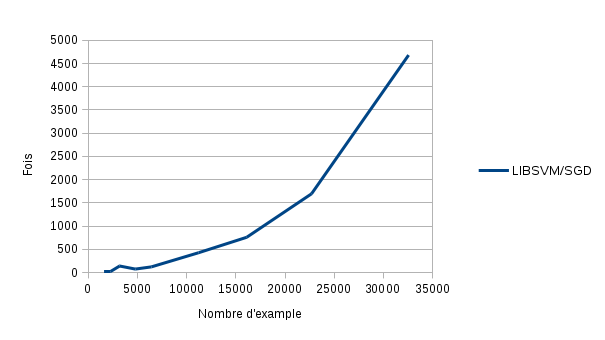
\includegraphics[width=150mm]{images/res}
\caption{Comparaison de la vitesse entre LibSVM et SGD binaire}
\label{fig:res}
\end{figure}

\pagebreak
Par rapport au table \ref{tab:svmsgd}, nous trouvons que le taux de classification du SGD et de la LibSVM est presque pareil tandis que le temps d'apprendre est différent. La vitesse du SGD est très vite que la vitesse de la LibSVM. Cet avantage du SGD est plus clair quand le nombre d'exemples d'apprentissage augmente. Cette chiffre est démontrée dans la colonne 7 de table \ref{tab:svmsgd} ou aussi dans le figure \ref{fig:res}.\\

Les données que nous avons utilisé ont 123 caractéristiques. Nous trouvons que quand le nombre d'exemple est de 1,605, l'algorithme SGD est plus vitesse que la LibSVM de 10 fois, mais quand le nombre d'exemple de 32,561, le SGD plus vitesse que la LibSVM 4,682 fois. Ce chiffre confirme que le SGD est beaucoup plus vitesse que la LibSVM, surtout pour les grandes données. Donc, l'algorithme SGD s'adapte mieux au problème de classification d'image dont la base de données est très grande. En raison de son avantage, nous voulons le développer pour qu'elle puisse résoudre le problème de classification multi-classes afin d'utiliser dans le domaine de classification d'images.

\section{MC-SGD pour la classification multi-classes}
\begin{itemize}
\item Protein : 3 classes, 17000 exemples, 357 caractéristiques
\item Mnist : 10 classes, 60000 exemples, 780 caractéristiques
\item SVM : function linéaire
\item SGD : -iter 500 -k 100 -lambda 0.05
\end{itemize}

\begin{table}[h]
\begin{center}
    \begin{tabular}{ | c | c | c | c | c | c | c | c |}
    \hline
    Données & SVM(\%) & 1-vs-all(\%) & 1-vs-1(\%) & SVM(s) & 1-vs-all(s) & 1-vs-1(s) & $\frac{SVM(s)}{SGD(s)}$ \\ \hline
    
    Protein & 68.23 & 68.41 & 69.10 & 551 & 0.20 & 0.19 & \textbf{2755} \\ \hline
    
    Mnist & 86.92 & 86.46 & 89.71 & 2810 & 0.72 & 4.23 & \textbf{3902.8} \\ \hline
    
    \end{tabular}
\end{center}
\caption{Comparaison entre LIBSVM et MC-SGD parallèle}
\label{tab:pmcsvm}
\end{table}

En générale, le résultat de classification du MC-SGD ne meilleure pas quand on compare avec la LibSVM. Par contre, le temps d'apprendre est beaucoup plus vite que la LibSVM pour le problème de classification multi-classes. La table \ref{tab:pmcsvm} est une preuve.
Pour le MC-SGD, nous trouvons que le résultat de classification de la version one-vs-one est un peu mieux que la version one-vs-all. Le temps  d'apprentissage de deux options est presque pareil pour le problème de 3 classes. Par contre, pour le problème de 10 classes, la version one-vs-one est plus lent que la version one-vs-all 5.8 fois. Ce chiffre va augmenter très vite quand le nombre de classes augmente. Pendant ce stage, nous nous concentrons à développer un algorithme qui peut améliorer le temps du SVM, donc, nous trouvons que la version one-vs-all est un bon choix. Pour les tests suivants, nous ne faisons que la comparaison entre la version one-vs-all du MC-SGD avec la LibSVM.

\section{MC-SGD pour la classification d'images}
Comme nous avons parlé dans le processus, notre processus pour la classification d'images comprend 3 étapes principales : extraction des descripteurs avec le descripteur SIFT, construit le dictionnaire avec la méthode K-moyenne et l'apprentissage automatique pour la classification avec la méthode MC-SGD. Dans la partie précédente nous avons présenté le résultat de l'algorithme MC-SGD (l'étape 3, l'étape d'apprentissage automatique) avec la base de données existante. Maintenant, nous appliquons la méthode Sac de Mots pour préparer les entrées pour l'algorithme MC-SGD avec les bases d'images pour voir si la méthode MC-SGD s'adapte pour le problème de classification d'images.
\begin{itemize}
\item SVM : function linéaire
\item SGD : -iter 1000 -k 10 -lambda 0.6
\end{itemize}

\begin{table}[h]
\begin{center}
    \begin{tabular}{ | c | c | c | c | c | c |}
    \hline
    Données & SVM(\%) & SGD(\%) & SVM(s) & SGD(s) & $\frac{SVM(s)}{SGD(s)}$ \\ \hline

    Cal 101 & 61.52 & 65.12 & 2873 & 106.95 & \textbf{26.9} \\ \hline
    
    Cal 7 3D & 91.52 & 88.3 & 113.4 & 0.81 & \textbf{140} \\ \hline 

    ImgNet 3d & 76.54 & 75.8 & 144 & 0.90 & \textbf{160} \\ \hline
    
    ImgNet & 84.08 & 86.58 & 327 & 1.64 & \textbf{199.4} \\ \hline
    
    \end{tabular}
\end{center}
\caption{Comparaison entre LIBSVM et MC-SGD parallèle pour la classification d'images}
\label{tab:pimgclasssvm}
\end{table}

Le tableau \ref{tab:pimgclasssvm} montre que le pourcentage de classification de la LibSVM est presque égale au MC-SGD. Par contre, la LibSVM est plus lent que le MC-SGD de 26 à 199 fois. Nous rappelons que la LibSVM utilise l'option one-vs-one et le MC-SGD utilise l'option one-vs-all. Donc, si la base d'image augmente plus de catégories (le nombre de classes), l'algorithme MC-SGD sera plus vitesse si l'on compare avec l'algorithme de la LibSVM.

%\pagebreak
Pour être facile de faire la comparaison sur la vitesse entre notre algorithme et la LibSVM, nous vous montrons la graphique \ref{fig:res1} (le taux de SVM/MC-SGD)
\begin{figure}[H]
\centering
\includegraphics[width=150mm]{images/res1}
\caption{Comparaison de SVM et MC-SGD (SVM/MC-SGD)}
\label{fig:res1}
\end{figure}

Non seulement plus vite que le SVM quand le nombre de classes augmente, mais aussi sur le nombre d'exemple d'apprentissage. La graphique ci-dessus peut montrer ce que nous expliquons. Le taux de temps de SVM/MC-SGD augmente selon le nombre d'exemple très claire dans cette graphique. Précisément, quand le nombre d'exemple de 1515, ce taux est de 26.9 mais ce taux est de 199.4 quand le nombre d'exemple est de 60000. La raisons est que notre algorithme n'a pas besoin de prendre tous les exemples pour l'apprentissage.\\


\cleardoublepage
\phantomsection
\addcontentsline{toc}{chapter}{Conclusion et perspectives}
\chapter*{Conclusion et perspectives}
\label{chap:con}
Se basant sur la méthode SVM, une méthode très populaire dans le domaine d'apprentissage automatique, les auteurs ont développé Pegasos \cite{sss07} utilisant le SGD binaire. En générale, la méthode Pegasos n'est pas meilleure que la méthode SVM sur la classification car le SGD est une version simple du SVM où l'on ne doit pas résoudre le problème de programme quadratique. Se basant sur SGD binaire, nous avons développé notre algorithme pour que SGD s'adapte bien au problème de multi-classes. Nous avons implémenté avec toutes les deux options possibles one-vs-one et one-vs-all. Pour le problème de classification de multi-classes avec one-vs-all, le SGD Pegasos trouve le problème de balancé. Pour cette raison, nous avons fait la échantillonnage et l'équilibra de la méthode SGD Pegasos. Dans cette recherche, nous ne faisons pas le point sur le résultat de classification, mais sur la vitesse de classification sur les bases d'images réelles. Donc, le MC-SGD s'adapte bien. Pour étudier notre algorithme, nous avons développé MC-SGD-Toy.\\

Bien que le MC-SGD a des avantages de la vitesse, cette méthode soit difficile de choisir des paramètres entrées tel que le nombre d'itération, lamda. Dans l'avenir, nous étudierons pour chercher des paramètres optimales de la méthode. Nous testerons aussi des bases d'images plus grandes tel que ImageNet. Nous développerons pour le SGD s'adapte aux autres domaines, tel que à la classification de vidéos.

\cleardoublepage
\phantomsection
\cleardoublepage
%\pagebreak
\phantomsection
\addcontentsline{toc}{chapter}{Bibliographie}
\begin{thebibliography}{99}

\bibitem{low99} David G. Lowe, \emph{Object Recognition from Local Scale-Invariant Features,} In proceeding of the 7th International conference of computer vision, pages 1150 - 1157, Corfou, Grèce, 1999.

\bibitem{sss07} Shalev-Shwartz, S.Singer, Y.Srebro, \emph{Primal esti-mated sub-gradient solver for svm.}, Proceedings of the Twenty-Fourth International Conference Machine Learning. pp. 807–814, ACM (2007).

\bibitem{svmdatamul}\emph{LIBSVM Data : Classification (Multi-class)},\ \url{<http://www.csie.ntu.edu.tw/~cjlin/libsvmtools/datasets/multiclass.html}

\bibitem{khang09} PHAM Nguyen Khang, \emph{Analyse factorielle des correspondances pour l'indexation et la recherche d'information dans une grande base de données d'image}, thèse IRISA, 2009.

\bibitem{sm97} C.Schmid and R.Mohr, \emph{Local Greyvalue Invariants for Image Retrieval}, IEEE Transactions on Pattern Analysis and Machine Intelligence,530--534, 19, 5 (1997).

\bibitem{hs88} Chris Harris and Mike Stephens, \emph{A combined corner and edge de detector},  in Alvey Vision Conf., 1988, pp. 147 - 151.

\bibitem{dsh00} Y.Dufournaud, C.Schmid and R.Horaud, \emph{Matching Images with Different Resolutions}, in "International Conference on Computer Vision and Pattern Recognition (CVPR '00) 1 (2000) 612--618"

\bibitem{lin98} Tony Lindeberg, \emph{Feature Detection with Automatic Scale Selection,} Technical report ISRN KTH/NA/P–96/18–SE, May 1996, Revised August 1998. Int. J. of Computer Vision, vol 30, number 2, 1998. (In press).

\bibitem{nk13} T-N DO, N-K PHAM, \emph{Phan lop anh voi giai thuat giam gradient ngau nhien da lop,} Magasin Cantho university, 29 (2013).

\bibitem{ms01} K.Mikolajczyk and C.Schmid, \emph{Indexing based on scale invariant interest points}, in "Computer Vision, 2001. ICCV 2001. Proceedings. Eighth IEEE International Conference on  (Volume:1 )", pages 525 - 531, 2001.

\bibitem{low04} David G. Lowe, \emph{Distinctive Image Features from Scale-Invariant Keypoints}, International journal of computer vision, 60(2), 91 - 110, 2004.

\bibitem{bmp02} S.Belongie, J.Malik and J.Puzicha, \emph{Shape matching and object recognition using shape contexts}, in "Pattern Analysis and Machine Intelligence, IEEE Transactions on  (Volume:24 ,  Issue: 4 )", pages 509 - 522, 2002.

\bibitem{ks04} Yan Ke and Rahul Sukthankar, \emph{PCA-SIFT: A More Distinctive Representation for Local Image Descriptors}, in "Computer Vision and Pattern Recognition", 2004.

\bibitem{ms05} K.Mikolajczyk and C.	Schmid, \emph{A performance evaluation of local descriptors}, in "Pattern Analysis and Machine Intelligence, IEEE Transactions on  (Volume:27 ,  Issue: 10 )", 2005.

\bibitem{mt10} Marco Treiber, \emph{An introduction to object recognition: selected algorithms for a wide variety of application}, ISBN 9781849962346, pages p. 147, 2010.

\bibitem{jm67} J.MacQueen, \emph{Some methods for classification and analysis of multivariate observations. Proceedings of 5th Berkeley Symposium on Mathematical Statistics and Probability}, Berkeley, University of California Press Vol.1, pp. 281-297 (1967).

\bibitem{jp98} J.Platt, \emph{Sequential Minimal Optimization: A Fast Algorithm for Training Support Vector Machines}, Microsoft Research Technical Report MSR-TR-98-14 (1998).

\bibitem{cl01} C.Chang and C.Lin, \emph{LIBSVM – a library for support vector machines}, http://www.csie.ntu.edu.tw/~cjlin/libsvm (2001).

\bibitem{ww99} J.Weston, C.Watkins\emph{Support vector machines for multi-class pattern recognition.}, Proceedings of the Seventh European Symposium on Artificial Neural Networks. pp. 219–224. (1999)

\bibitem{vv95} V.Vapnik, \emph{The Nature of Statistical Learning Theory.}, Springer, New York (1995).

\bibitem{vv82} V.Vapnik, et S. Kotz \emph{Estimation of Dependences Based on Empirical Data,} Springer Series in Statistics, 1982, ISBN 978-0387907338.

\bibitem{uk99} U.Krebel, \emph{Pairwise classification and support vector machines}, Support Vector Learning, Advances in Kernel Methods. pp.255–268. (1999).

\bibitem{bos07} A.Bosch, A.Zisserman and X.Munoz \emph{Scene
classification via pLSA.}, Proceedings of the European Conference on Computer Vision, pp. 517–530 (2006).

\bibitem{mq67} J.MacQueen \emph{Some methods for classification and analysis of multivariate observations.}, Proceedings of 5th Berkeley Symposium on Mathematical Statistics and Probability, Berkeley, University of California Press Vol.1, pp. 281-297 (1967).

\bibitem{khang} Nguyen-Khang Pham http://www.cit.ctu.edu.vn/~pnkhang/index-en.html, Can Tho University

\bibitem{svmdata1}\emph{LIBSVM Data: Classification (Binary Class)},\ \url{http://www.csie.ntu.edu.tw/~cjlin/libsvmtools/datasets/binary.html}

%\bibitem{ms02} K.Mikolajczyk, Detection of local features invariant to affine transformations, Ph.D. thesis, Institut National Polytechnique de Grenoble, France, 2002.

%\bibitem{yg07} J.Weston, C.Watkins\emph{Svm multiclasses.}, théorie et applications (2007)

\end{thebibliography}


\cleardoublepage  % \clearpage (if using single side)
\phantomsection
\addcontentsline{toc}{chapter}{\listfigurename} \raggedbottom \pagebreak \thispagestyle{empty}
\listoffigures

\cleardoublepage  % \clearpage (if using single side)
\phantomsection
\addcontentsline{toc}{chapter}{\listtablename} \raggedbottom \pagebreak \thispagestyle{empty}
\listoftables

\cleardoublepage  % \clearpage (if using single side)
\phantomsection
\renewcommand{\listalgorithmname}{Liste des algorithmes}
\addcontentsline{toc}{chapter}{\listalgorithmname} \raggedbottom \pagebreak \thispagestyle{empty}
\listofalgorithms
\addtocontents{loa}{\def\string\figurename{Algorithm}}

\end{otherlanguage}

\end{document}
